% standalone wrapper for a tikz picture
\documentclass[tikz,border=2pt]{standalone}
\usepackage{xcolor}
\usepackage{tikz}
\usetikzlibrary{shapes,arrows,positioning,shadows,patterns,arrows.meta,calc}
\definecolor{cwAlert}{RGB}{220,50,50}
\definecolor{cwFlow}{RGB}{50,120,220}
\definecolor{cwDecoy}{RGB}{120,180,50}
\definecolor{cwBorder}{RGB}{80,80,80}
\definecolor{ImperialBlue}{RGB}{0,62,116}
\definecolor{ImperialNavy}{RGB}{0,33,71}
\definecolor{ImperialLightBlue}{RGB}{155,203,235}
\begin{document}

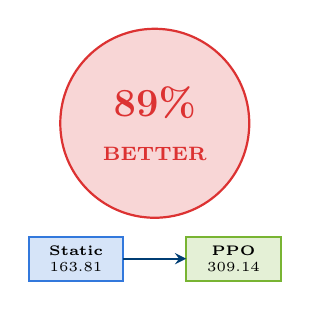
\begin{tikzpicture}[scale=0.8]
    \draw[fill=cwAlert!20, draw=cwAlert, thick] (0,0) circle (1.5);
    \node[align=center, font=\Large\bfseries] at (0,0) {\textcolor{cwAlert}{89\%}\\[-2pt]\textcolor{cwAlert}{\scriptsize BETTER}};
    
    \draw[fill=cwFlow!20, draw=cwFlow, thick] (-2,-2.5) rectangle (-0.5,-1.8);
    \node[align=center, font=\tiny] at (-1.25,-2.15) {\textbf{Static}\\163.81};
    
    \draw[fill=cwDecoy!20, draw=cwDecoy, thick] (0.5,-2.5) rectangle (2,-1.8);
    \node[align=center, font=\tiny] at (1.25,-2.15) {\textbf{PPO}\\309.14};
    
    \draw[-stealth, thick, ImperialBlue] (-0.5,-2.15) -- (0.5,-2.15);
\end{tikzpicture}
\end{document}
